% Chapter X

\chapter{StyleCheck: A Tool to Apply Style Guides}
\label{ch:stylecheck}

%----------------------------------------------------------------------------------------

\section{Style Guides}

\noindent Following the proposed methodology, translation theory was used as a basis to develop a \ac{CAT} tool that implements a \ac{SG}. \acp{SG} are collections of rules that serve to standardise linguistic content \parencite{vidal2013guia}. Within a language, many different ways of writing or expressing an idea exist. From the wide range of possibilities, dialects choose a subset, as do specific domains, genres, language academies and even individuals. Style guides aim to define a subset of language for use in a specific domain (such as style manuals for scientific writing) or most commonly for a specific entity \parencite{vidal2013guia}. In the latter type we can place \acp{SG} from the European Union, from Wikipedia or from newspapers and other publications. The idea is to guarantee that texts written by different authors conform to a set of rules so that they can be recognised as coming from a single entity, creating a specific ``voice'' of sorts. 

Style guides can be more or less restrictive, \ie aim to cover a larger or smaller subset of linguistic phenomena that need to be standardised. \aclp{CNL} can be considered an extreme form of \acp{SG} where basic syntax and constructions of a language are defined. Style guides tend to focus on formal aspects (such as punctuation and formatting), lexicon, specific linguistic constructions, etc. 

Style guides are essentially made up of rules. The structure of these rules is to identify a specific linguistic element (word, punctuation, structure, meaning, etc.) and offer the one or more ways in which it should be expressed, often giving examples of the ways in which it should not be expressed \parencite{vidal2013guia}. Thus, to apply style guide rules digitally requires a system that can detect the specific linguistic element and is able to transform it \parencite{vidal2013guia}.

It is worth mentioning that many style guides also include information not directly related to linguistic standardisation, such as legal considerations for journalists, encyclopaedic knowledge about a certain topic, how to use company software or insert certain symbols into a Word document, etc. This evidences the informal nature of style guides and the multiple aims they sometimes try to serve.

Style guides are an important skill a translator should learn as they are widely used when translating \parencite{washbourne2012style}. A problem for translators is that they may have to handle many different style guides, each for a specific client. In this context, it is easy to mix-up the rules or simply not bother reading through a large style guide for a small job: the time that would be invested in learning the guide's rules would far exceed the time spent on the translation itself. The proof-reader is then charged with ensuring style guide rules are applied during the revision phase.

StyleCheck aims to solve the problem. As translators work on a text, they will be offered suggestions when rules contained in a style guide haven't been applied. Then, they will be able to immediately solve the problem by applying them, which will reduce the time needed for proof-reading and the time spent learning a style guide.

%----------------------------------------------------------------------------------------

\section{Grammatical Framework}

\noindent StyleCheck is implemented using \ac{GF} \parencite{ranta2011gf}. \ac{GF} is a programming language and grammar formalism used to build multilingual grammar applications. \ac{GF} draws heavily from functional programming and from type theory. The real strength of \ac{GF} is the \ac{RGL} \parencite{ranta2009rgl}, which implements basic morphology and syntax for a number of languages. The \ac{RGL} provides a common, high-level \spacedlowsmallcaps{API} to use the syntax, allowing for fast multilingual application development. Relevant for StyleCheck is \ac{GF}'s tried and tested use in the field of \ac{CNL} \parencite{angelov2009cnl,kaljurand2013wiki,ranta2014embedded}.

Grammars in \ac{GF} are split into two parts: the abstract syntax and the concrete syntax. The abstract syntax is intended to represent semantics, while the concrete syntax (one for each language) links the abstract syntax to a particular string representation. More specifically, functions defined in the abstract syntax are mapped to linearizations in the concrete syntax. 

As an example, the abstract syntax funcion

\begin{lstlisting}[numbers=none]
fun AvoidSeasons_Hint : StyleHint ;
\end{lstlisting}

%\begin{minted}
%fun AvoidSeasons_Hint : StyleHint ;
%\end{minted}
%
%\begin{minted}{tex}
%fun AvoidSeasons_Hint : StyleHint ;
%\end{minted}

\noindent builds a record of type \texttt{StyleHint}. In the Spanish concrete syntax, this would be realised as:

\begin{lstlisting}[numbers=none]
lin AvoidSeasons_Hint = mkStyleHint "verano" "Don't use seasons";
\end{lstlisting}

\noindent where a \texttt{StyleHint} is a record built out of a season ``verano'' and the suggestion ``Don't use seasons''. When ``verano'' is encountered during parsing, a \texttt{StyleHint} is built and mapped to the abstract syntax function \texttt{AvoidSeasons\_Hint}. Then, from the abstract syntax tree representation a different concrete syntax can take the abstract function that was matched in the text and select from it only the suggestion text, which can then be output to the user.

This is a simplified view of how StyleCheck is designed, but it serves to illustrate the main idea: a text is parsed and any detected style rules are mapped to a style suggestion.


%----------------------------------------------------------------------------------------

\section{StyleCheck}

%------------------------------------------------
\subsection{Development Procedure}

\noindent The StyleCheck grammar was developed as follows. First, from each text to be used in the online experiment all Wikipedia style guide rules that could be applied to it were identified. Since the style guide refers to the Diccionario Panhispánico de Dudas \parencite{real2005dudas} for aspects not specifically mentioned in the style guide, it too was checked. The obtained rules were then classified as rules, hints or lookups in the following manner:

\begin{itemize}
    \item \textit{Style rules:} linguistic elements that have more than one possible forms, out of which one or more forms are approved by the style guide. For example, the correct spelling in Spanish of the capital of \spacedlowsmallcaps{UAE} is ``Abu Dabi'', not ``Abu Dhabi'' as in English.
    \item \textit{Style hints:} linguistic elements whose approved form is not self-evident and requires reasoning. Through the use of a suggestion, the translator can be made aware of the issue and decide whether action needs to be taken or not. For example, the Wikipedia style guide recommends not temporally locating events using only seasons, as the months they refer to differ in the Northern and Southern hemisphere of the Earth. In this case, all mentions of a season would trigger a suggestion for the translator to check this aspect.
    \item \textit{Style lookups:} the third possibility that was contemplated were style lookups. For some elements that have many possibile uses, such as full stops, commas or slashes, showing a suggestion every time they appear as would be the case with a style hint was deemed to be too annoying. Instead, style lookups would allow the translator to select one of these common elements and be taken shown the full range of possibilities. Thus, the translator would only lookup these elements on-demand, when he or she would consider it necessary.
\end{itemize}

Given that only one rule was classified as a style lookup (the use of the forward slash symbol), it was decided to apply it as a style hint instead and leave the lookup framework at the theoretical design stage to be implemented in future work. The forward slash only appeared once in one of the texts, so it didn't risk being annoying as would be the case if it were a comma or a full stop.

Rules were implemented as a record with fields for optional forms, approved forms and the hint (\autoref{lst:records}). Style hints and lookups contained all the fields in a rule, except for the \texttt{approved} field. All of these fields were of type \texttt{Chunk}, which is simply defined as a string.

\begin{lstlisting}[caption={Record structure for the rule types},label=lst:records]
StyleRule = {approved,options,hint : Chunk} ;
StyleHint = {options,hint : Chunk} ;
StyleLookup = {options,hint : Chunk} ;
\end{lstlisting}

The main problem with developing style rules and hints is identifying the range of options that can be encountered in a text. Not only is it necessary to think about what possible forms a rule can manifest itself into, but misspellings of these forms also need to be taken into account. In order to help in this effort, several helper functions were defined which generated options on the basis of including full stops or not (to create the possible misspellings for ordinal abbreviations in Spanish: 7.º and 7º), including a space between compounds or not, etc. The \texttt{approved} and \texttt{options} themselves were implemented either as strings or using types and functions defined in the Spanish \spacedlowsmallcaps{RGL}, allowing for the full morphological forms to be matched.

Lastly, we turn to the hint format. \textcite{vidal2013guia} found that the rules contained in \acp{SG} come in all shapes and sizes. Some are included as part of a text and are written in a narrative style, others are included as entries in a dictionary format referring to a specific keyword. The Wikipedia style guide takes the narrative approach, justifying why many of the decisions are made and explaining a lot of the concepts. So as to not introduce another variable to analyse, for this thesis the hints were taken as-is or with very minimal editing from the guide and shown directly to the translator. This generated suggestions that sometimes spanned several lines of text. A better approach would have been to rework the suggestions into one-liners apt for a quick glance, and provide an option to further expand on the descriptions or reasoning behind the rules if desired by the translator.

%------------------------------------------------

\subsection{Grammar Structure}

\noindent Despite the small scale of the grammar and the few rules that were implemented, the full file and module structure of a larger grammar was used in order to show how a full system would be implemented. \autoref{fig:grammar_full} represents how the full grammar was built.

\begin{figure}[h]
\myfloatalign
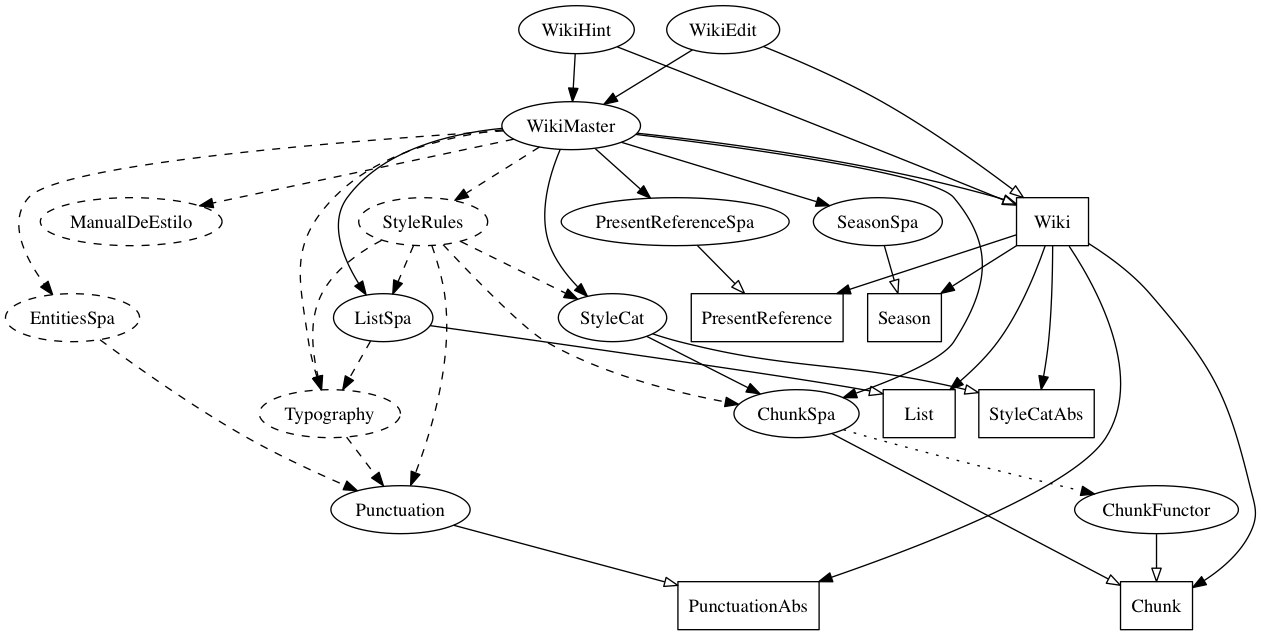
\includegraphics[width=\textwidth]{img/grammar/grammar_full}
\caption{Full module structure and dependencies that make up StyleCheck}
\label{fig:grammar_full}
\end{figure}

\graffito{Code for the three main modules \texttt{Wiki}, \texttt{WikiMaster} and \texttt{WikiHint} can be found in \autoref{app:code}}
First, we will describe the main grammar components. This subset of the full grammar is shown in \autoref{fig:grammar_simple}. The main abstract syntax module is \texttt{Wiki}, which contains a function for each of the rules (\autoref{lst:wiki}). This abstract syntax has three corresponding concrete syntax modules: \texttt{WikiMaster}, \texttt{WikiHint} and \texttt{WikiEdit}. \texttt{WikiMaster} (\autoref{lst:wikimaster}) contains the main parsing mechanics. In it, each abstract syntax function is linearised into the required type: \texttt{StyleRule}, \texttt{StyleHint} or \texttt{StyleLookup}:

\begin{figure}[h]
\myfloatalign
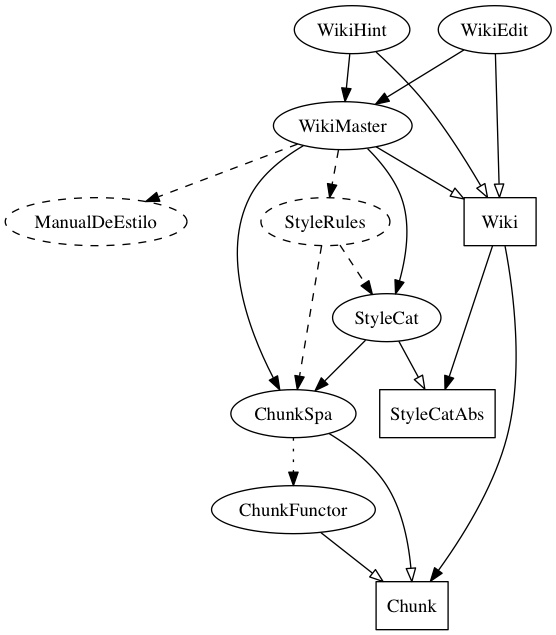
\includegraphics[width=0.8\textwidth]{img/grammar/grammar_simple}
\caption{Main StyleCheck modules and dependencies}
\label{fig:grammar_simple}
\end{figure}

\begin{itemize}
    \item These three types are defined in the abstract syntax \texttt{StyleCatAbs} and in the concrete \texttt{StyleCat}. 
    \item Convenience functions to build these types are provided in the resource module \texttt{StyleRules}.
    \item To build the options, \texttt{WikiMaster} uses the necessary components from the Spanish \spacedlowsmallcaps{RGL} (not shown in \autoref{fig:grammar_simple}). 
    \item The text for the style hints is contained in \texttt{ManualDeEstilo}.
\end{itemize}

\noindent Once the required style types are built, \texttt{WikiMaster} builds \texttt{Chunk} types out of them. The idea is that when parsing a sentence, once or more \texttt{Chunk}s (each corresponding to a style rule, hint or lookup) are identified, appended together, and output as the result of the parse. To acheive this, StyleCheck makes use of the chunking types and functions used in the Wide-Coverage Translator being built upon \ac{GF} \parencite{ranta2014embedded}. The abstract syntax for these types is \texttt{Chunk}, and the concrete is \texttt{ChunkSpa}. Finally, the top level type, a \texttt{Phr}, is built out of one or more \texttt{Chunk}s.

To sum up, the parsing mechanics are as follows:

\begin{enumerate}
    \item A style rule is matched and a style rule, hint or lookup type is built.
    \item \texttt{WikiMaster} selects the \texttt{options} from the style record and builds a \texttt{Chunk} out of them.
    \item Through the functions included in \texttt{ChunkSpa}, a \texttt{Phr} type is built, which is the top level category in the grammar.
    \item The tree constructed until now is linearised using \texttt{WikiHint}. This concrete syntax selects the \texttt{hint} field from the style type record, resulting in the hint text being output.
    \item A simple regex extracts all the hints from the output (hints are delimited with \texttt{|||} to make this task easy). Any non-matches will simply return the original token.
\end{enumerate}

The additional modules shown in \autoref{fig:grammar_full}, such as \texttt{ListSpa} or \texttt{Typography} ease the task of writing style rules. They mainly contain functions and opers related to a specific rule in StyleCheck.

Finally, there is one extra concrete syntax that isn't used in this thesis. The \texttt{WikiEdit} shows how an automatic post-editing tool would work. It simply selects the \texttt{approved} field from the style record instead of the hint for \texttt{StyleRule}s (the only types that have an approved field). This kind of funtionality for \ac{CAT} tools needs further thought and development, since it could be very confusing for translators to find parts of their texts changed without warning.

\section{Intrinsic evaluation}

\noindent In order to develop the grammar, the possible options for each rule had to be thought out. A test sentence was created for each option, together forming a small corpus. The grammar was developed so that it would generate the correct output on the small corpus of options. This was evaluated by having \ac{GF} parse the sentences and check that the grammar brings up the correct style hint.

Intrinsic evaluation as described will perform well on the corpus, but some cases can fall through the net. Looking into the final translations carried out by the experiment's participants, two cases were found of options that the grammar did not detect:

\begin{itemize}
    \item Rule 2.B (\autoref{lst:wiki}, \autoref{lst:wikimaster}) states that temporal references should not use the moment of enunciation as reference point. For example, in ``Her most recent work'', \textit{recent} refers to the moment of enunciation. Future readers may consider \textit{recent} as a different time period than the writer, so it should be avoided. Even though StyleCheck was developed with several adverbial time markers that refer to the moment of enunciation (\textit{recientemente}, \textit{hoy}, \textit{ahora}, etc.), one participant used an adjective form instead (``la más reciente''), which was not in the grammar and did not generate a hint.
    \item Another simpler case is that of the \spacedlowsmallcaps{USA}. The acceptable forms in Spanish are \spacedlowsmallcaps{EE. UU.} (with a space) or \spacedlowsmallcaps{EUA}. Several non-approved options were generated, such as \spacedlowsmallcaps{EE.UU.} (without a space) or \spacedlowsmallcaps{USA}. One participant, however, used the form \spacedlowsmallcaps{EEUU}, which was not in the grammar and would not have triggered a style hint.
\end{itemize}

The advantage of having built a prototype is once again clear. The previous issues can be solved straight away and directly integrated into a future version of StyleCheck.
